\documentclass[11pt]{article}
\usepackage[utf8]{inputenc}
\usepackage[english, ngerman]{babel}
\usepackage{amsmath,amsthm,verbatim,amssymb,amsfonts,amscd}
\usepackage{enumerate}
\usepackage{listings}
\usepackage{courier}
\usepackage{graphicx}
\usepackage{epstopdf}
\usepackage[margin=1in]{geometry}
\lstset{
  numbers=left,
  language=C,
  basicstyle=\footnotesize\ttfamily,
  breaklines=true,
  morekeywords={function, NIL}
}
\newcommand{\abs}[1]{\left| #1 \right| }
\setlength{\parindent}{0pt} 

\author{
  Felix Schrader, 3053850 \\ 
  Jens Duffert, 2843110 \\
  Eduard Sauter, 3053470
}
\title{Datenstrukturen und Algorithmen: Haus\"ubung 10}
\begin{document}
\maketitle
\subsection*{Aufgabe 1}
Allgemein gilt für einen B$^{+}$-Baum:\\
\begin{enumerate}
\item
	- Die Wurzel de Baums hat zwischen 1 und 2m Schlüssel
\item
	- Alles anderen internen Knoten haben zwischen m und 2m Schlüssel
\item
	- Alle Wege von der Wurzel zu einem Blatt haben die gleiche Länge
\end{enumerate}
	
Der erste Baum verstößt gegen den dritten Punkt, da nicht alle Wege von\\
den einzelnen Blättern zur Wurzel gleich lang sind. Daher ist dies kein Baum
der Ordnung 2.\\
Der zweite Baum ist ein B$^{+}$ der Ordnung 2, da er alle oben genannten 
Bedingungen erfüllt.
\newpage
\subsection*{Aufgabe 2}
\begin{figure}[h!]
  \centering
  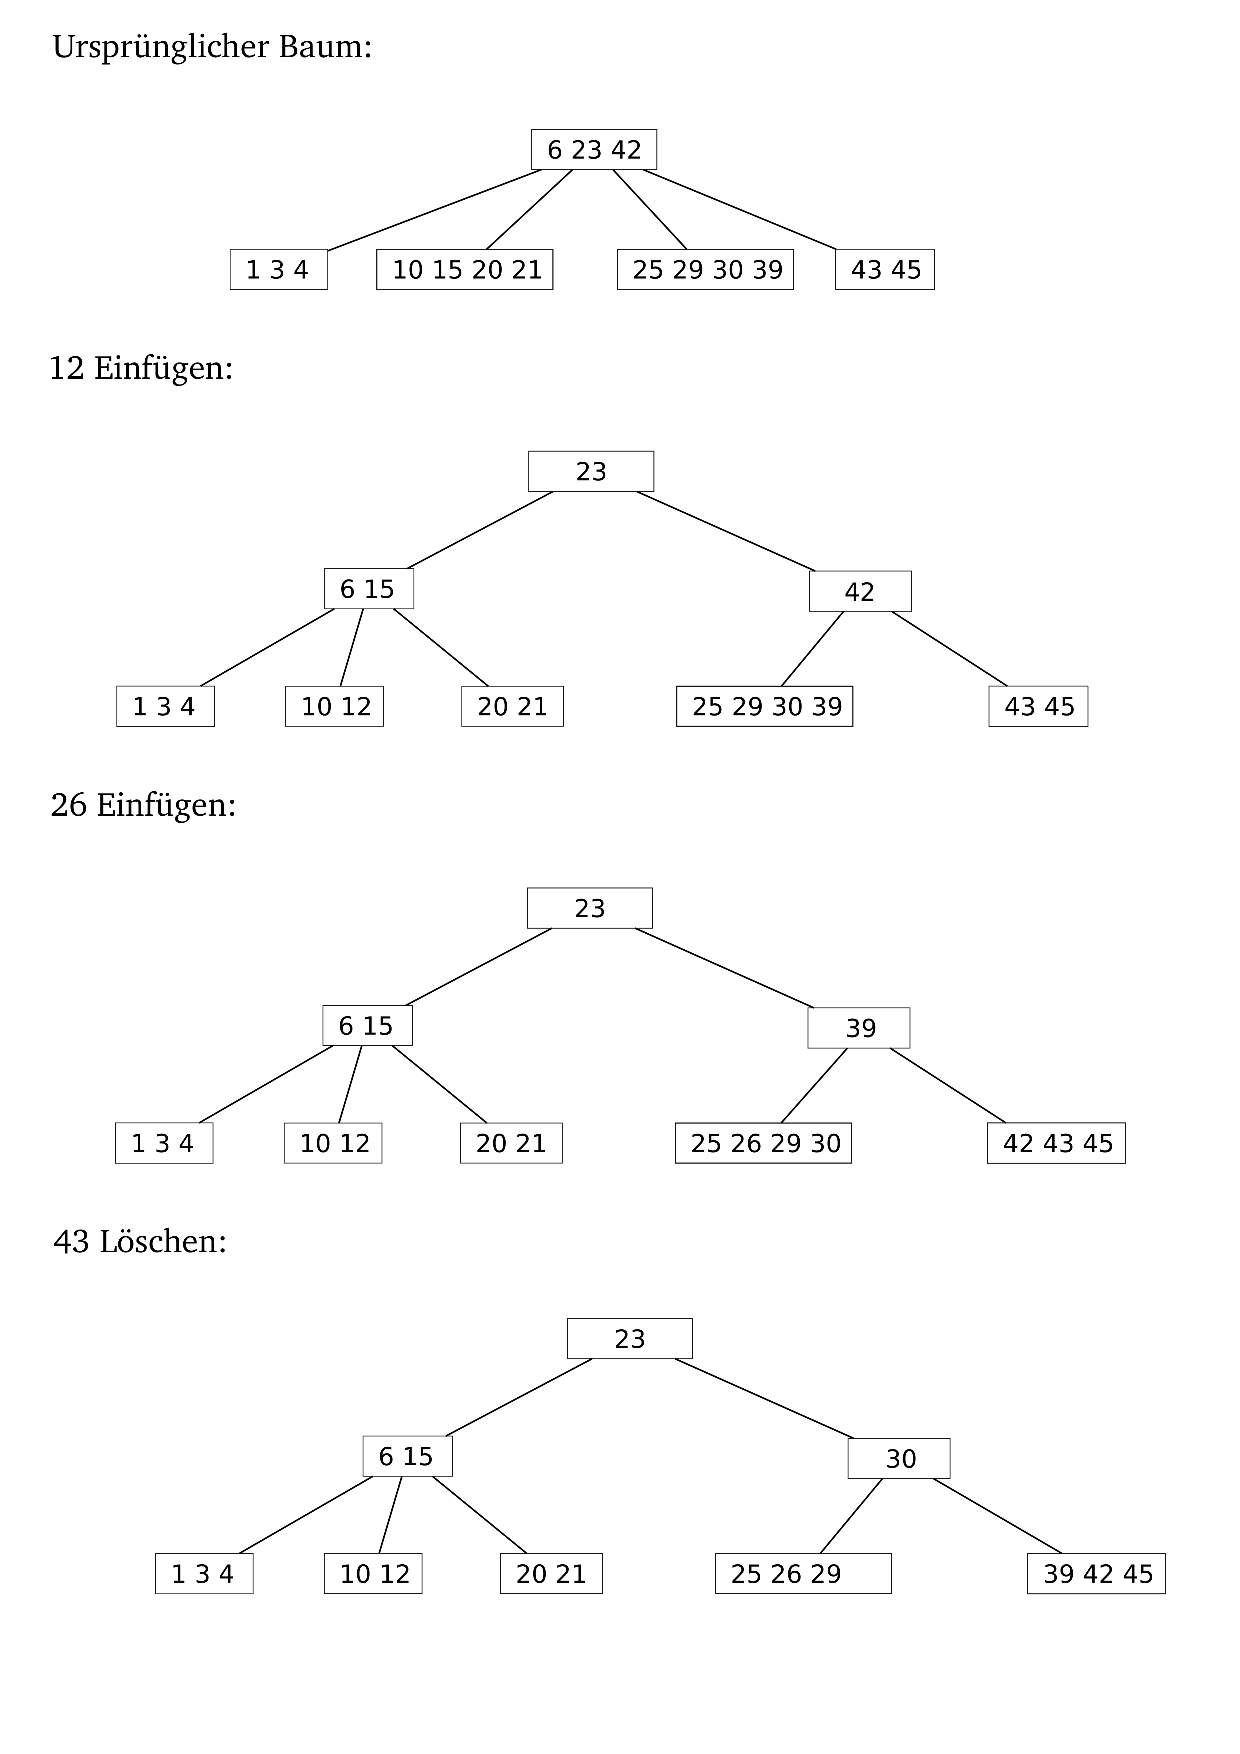
\includegraphics[width=0.9\textwidth]{b+tree_insert_delete}
  \label{fig:tree_insert_delete}
\end{figure}
\newpage
\subsection*{Aufgabe 3}
In einem B$^+$-Baum der Ordnung 2 haben alle Knoten nach Definition maximal vier
Schlüssel. Ein interner Knoten hat daher maximal fünf Nachfolger. Der
abgebildete Baum hat die Höhe 2, wenn man die Höhe nicht ändert passen also
maximal
\begin{align*}
  4 + 5 \cdot 4 + 5 \cdot 5 \cdot 4 = 124
\end{align*}
Werte in den Baum. In dem Baum in der Aufgabe sind bereits 19 Schlüssel, man
kann also insgesamt 105 Werte einfügen ohne die Höhe des Baumes zu ändern.
\end{document}
